% \documentclass[russian,14pt,floatsection,nocolumnsxix, nocolumnxxxii,nocolumnxxxi]{eskdtext}
\usepackage[utf8x]{inputenc}

% закомментировать для рамок 
\usepackage[numbertop, numbercenter]{eskdplain}

% для объединения строк в таблице
\usepackage{multirow}



% для размера колонок
\usepackage{tabularx}
\usepackage{lscape}
\newcolumntype{n}{>{\hsize=.4\hsize}X}
\newcolumntype{m}{>{\hsize=.2\hsize}X}


\usepackage{setspace}
\onehalfspacing % полуторный интервал для всего текста

% - Подключаем шрифты из пакета scalable-cyrfonts-tex
\usepackage{cyrtimes}

% - Отступ красной строки
\setlength{\parindent}{1.25cm}

% - Убирает точку в списке литературы
\makeatletter
\def\@biblabel#1{#1 }

% ограничение для оглавления
%\usepackage{tocvsec2}
\setcounter{tocdepth}{2}

% - Точки для всех пунктов в оглавлении
\renewcommand*{\l@section}{\@dottedtocline{1}{1.5em}{2.3em}}
\renewcommand*{\l@subsection}{\@dottedtocline{1}{1.5em}{2.3em}}
% \renewcommand*{\l@subsubsection}{\@dottedtocline{1}{1.5em}{2.3em}}

% - Для переопределения списков
\renewcommand{\theenumi}{\arabic{enumi}}
\renewcommand{\labelenumi}{\theenumi)}
\makeatother

\usepackage{enumitem}
\setlist{nolistsep, itemsep=0.3cm,parsep=0pt}

% - ГОСТ списка литературы
\bibliographystyle{utf8gost705u}


% - Верикальные отступы заголовков 
\ESKDsectSkip{section}{1em}{1em}
\ESKDsectSkip{subsection}{1em}{1em}
\ESKDsectSkip{subsubsection}{1em}{1em}

% - Изменение заголовков
\usepackage{titlesec}
\titleformat{\section}{\normalfont\normalsize\centering}{\thesection}{1.0em}{}
\titleformat{\subsection}{\normalfont\normalsize\centering}{\thesubsection}{1.0em}{}
\titleformat{\subsubsection}{\normalfont\normalsize\centering}{\thesubsubsection}{1.0em}{}
\titleformat{\paragraph}{\normalfont\normalsize\centering}{\theparagraph}{1.0em}{}

% - Оставим место под ТЗ 
\setcounter{page}{1}

% - Для больших таблиц
\usepackage{longtable}
\usepackage{tabularx}
\renewcommand{\thetable}{\thesection.\arabic{table}}

% - Используем графику в документе
\usepackage{graphicx}
\graphicspath{{images/}}
\renewcommand{\thefigure}{\thesection.\arabic{figure}}
% to have figure on top
%
\makeatletter
\setlength{\@fptop}{0pt}
\makeatother

% - Счётчики
\usepackage{eskdtotal}

% - Выравнивание по ширине
\sloppy

% - Разрешить перенос двух последних букв слова
\righthyphenmin=2

% - Оформление списков
\RequirePackage{enumitem}
\renewcommand{\alph}[1]{\asbuk{#1}}
\setlist{nolistsep}
\setitemize[1]{label=--, fullwidth, itemindent=\parindent, 
  listparindent=\parindent}% для дефисного списка
\setitemize[2]{label=--, fullwidth, itemindent=\parindent, 
  listparindent=\parindent, leftmargin=\parindent}
\setenumerate[1]{label=\arabic*), fullwidth, itemindent=\parindent, 
  listparindent=\parindent}% для нумерованного списка
\setenumerate[2]{label=\alph*), fullwidth, itemindent=\parindent, 
  listparindent=\parindent, leftmargin=\parindent}% для списка 2-ой ступени, который будет нумероваться а), б) и т.д.
  
% - Оформляем листинг кода (не использовать комментарии на русском!)
\usepackage{listings}  
\lstset{basicstyle=\ttfamily\scriptsize}
\lstset{extendedchars=\true}

% - выводим текст как есть с размером шрифта scriptsize
\makeatletter
\def\verbatim{\scriptsize\@verbatim \frenchspacing\@vobeyspaces \@xverbatim}
\makeatother

% - Вставка pdf
\usepackage[enable-survey]{pdfpages}

%межстрочный интервал
\usepackage{setspace}
\linespread{1.5}

%фамилии для рамок
\author{\ESKDfontII Мейта М.В.}
\ESKDchecker{\ESKDfontII Глухарева С.В.}
\ESKDnormContr{\ESKDfontII Якимук А.Ю.}
\ESKDapprovedBy{\ESKDfontII Шелупанов А.А.}
\ESKDcolumnI{\ESKDfontIII Технико-экономическое обоснование дипломной работы}
\ESKDcolumnIX{\ESKDfontIII ТУСУР, ФБ, каф.~КИБЭВС, гр.~722}
\ESKDsignature{КИБЭВС.58.29.29 ПЗ}

% 
% \begin{document}
%  
% \setcounter{page}{33}
% \setcounter{section}{11}
% 
% \ESKDstyle{formIIab}
% % \ESKDputOnStyle{formII}{frame}{\renewcommand{\ESKDchecker}{\ESKDfontII Глухарева С.В.}}
% \ESKDthisStyle{formII}
% 
% \renewcommand{\ESKDcolumnI}{\ESKDfontIII Технико-экономическое обоснование дипломной работы}
% 
% 
% \section{Технико-экономическое обоснование дипломной работы}
% \subsection{Обоснование актуальности дипломной работы}
% 
% Вследствие активного развития информационных технологий возрастает и количество преступлений в информационной сфере.
% Зачастую злоумышленники, как внешние, так и внутренние, используют самостоятельно разработанные программы для осуществления 
% атак на информационные ресурсы.
% Системы, способные идентифицировать разработчиков вредоносного ПО, могут внести существенный вклад в развитие компьютерной
% криминалистики, а также оказывать помощь в исследовании вопросов интеллектуальной собственности среди разработчиков программного
% обеспечения.
% 
% Цель настроящей дипломной работы --- разработать ПО, способное идентифицировать автора программы по исходному коду, с перспективой его
% дальнейшего применения в борьбе с киберпреступностью, в области лицензионных, патентных, и иных судебных разбирательств.
% 
% 
% \subsection{Организация и планирование работы}
% 
% Судент может быть принят на работу техником. 
% Должностной оклад техника составляет 4400 рублей в месяц.
% Стоимость одного часа работ руководителя с ученой степенью кандидата наук и должностью доцента
% согласно коллективному договору ТУСУР на 2016-2019 годы
% равна 230 рублей.    
% 
% Согласно выделенным этапам работы расчитывется трудоемкость 
% выполненных работ (табл.~\ref{tab:job_is_done_1}), а также строится диаграмма
% Ганта (рис.~\ref{grantt:grantt}), отображающего затраты времени на выполнение дипломной работы всеми
% участниками, представленная в приложении Ж.

%%%%%%%



\setcounter{section}{12}
\setcounter{subsection}{2}
\setcounter{figure}{0}

\begin{table}[ht!]
\caption{Трудоемкость выполненных работ}
\centering
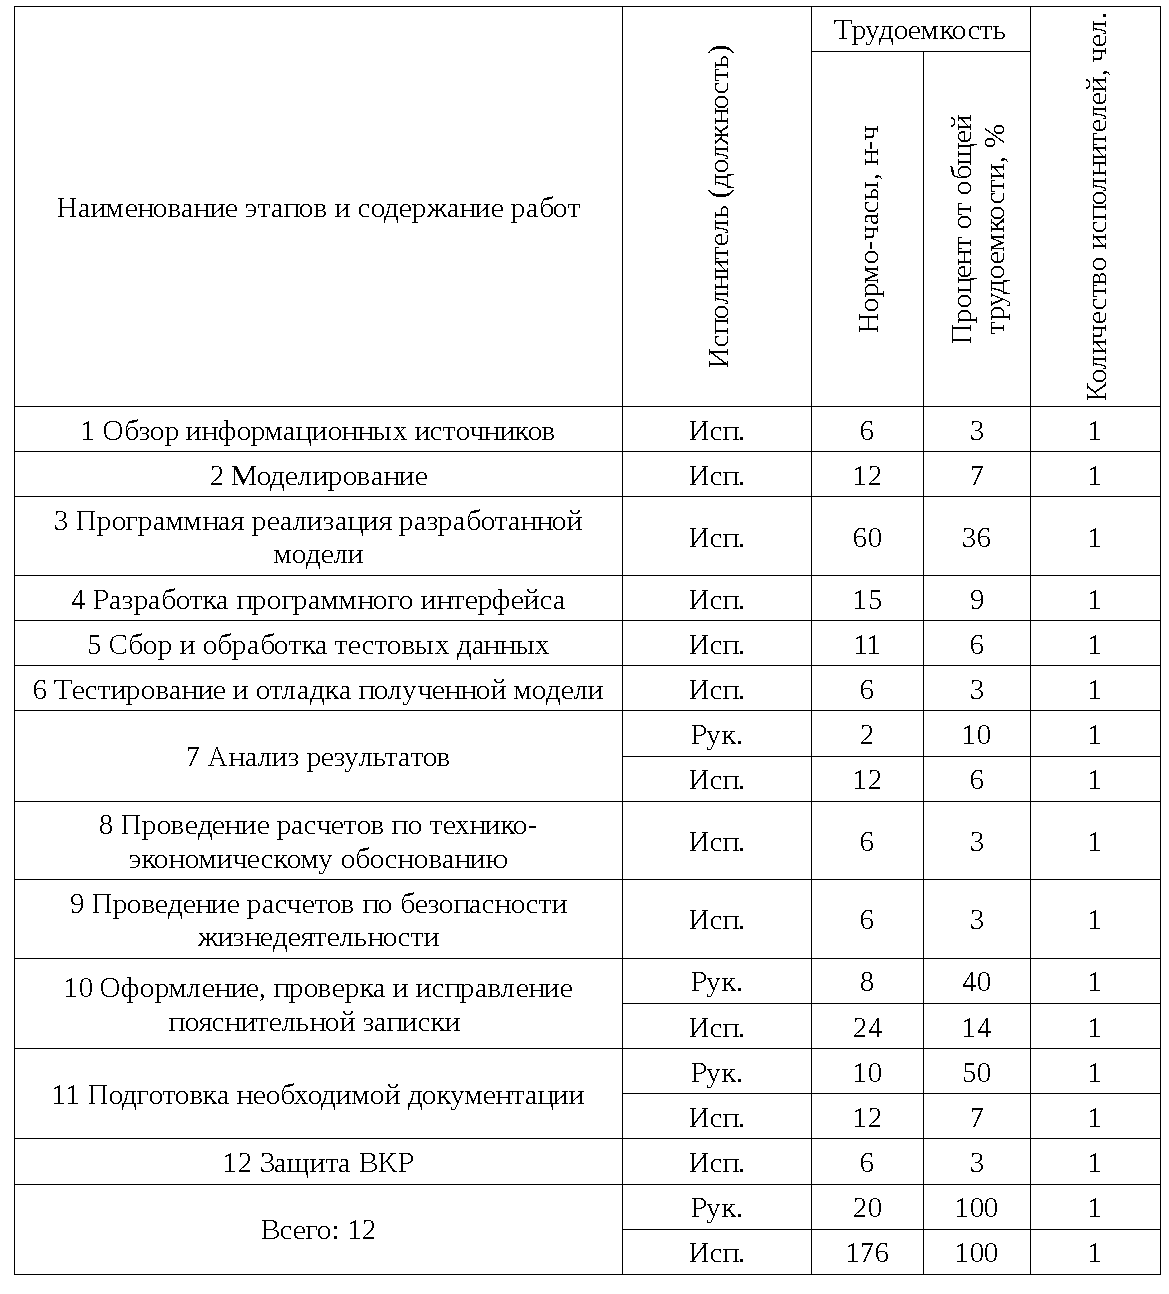
\includegraphics[page=1, width=1\linewidth]{tables/economics/schedule.pdf}
\label{tab:job_is_done_1}
\end{table}


\clearpage
\begin{figure}[h!]
\center{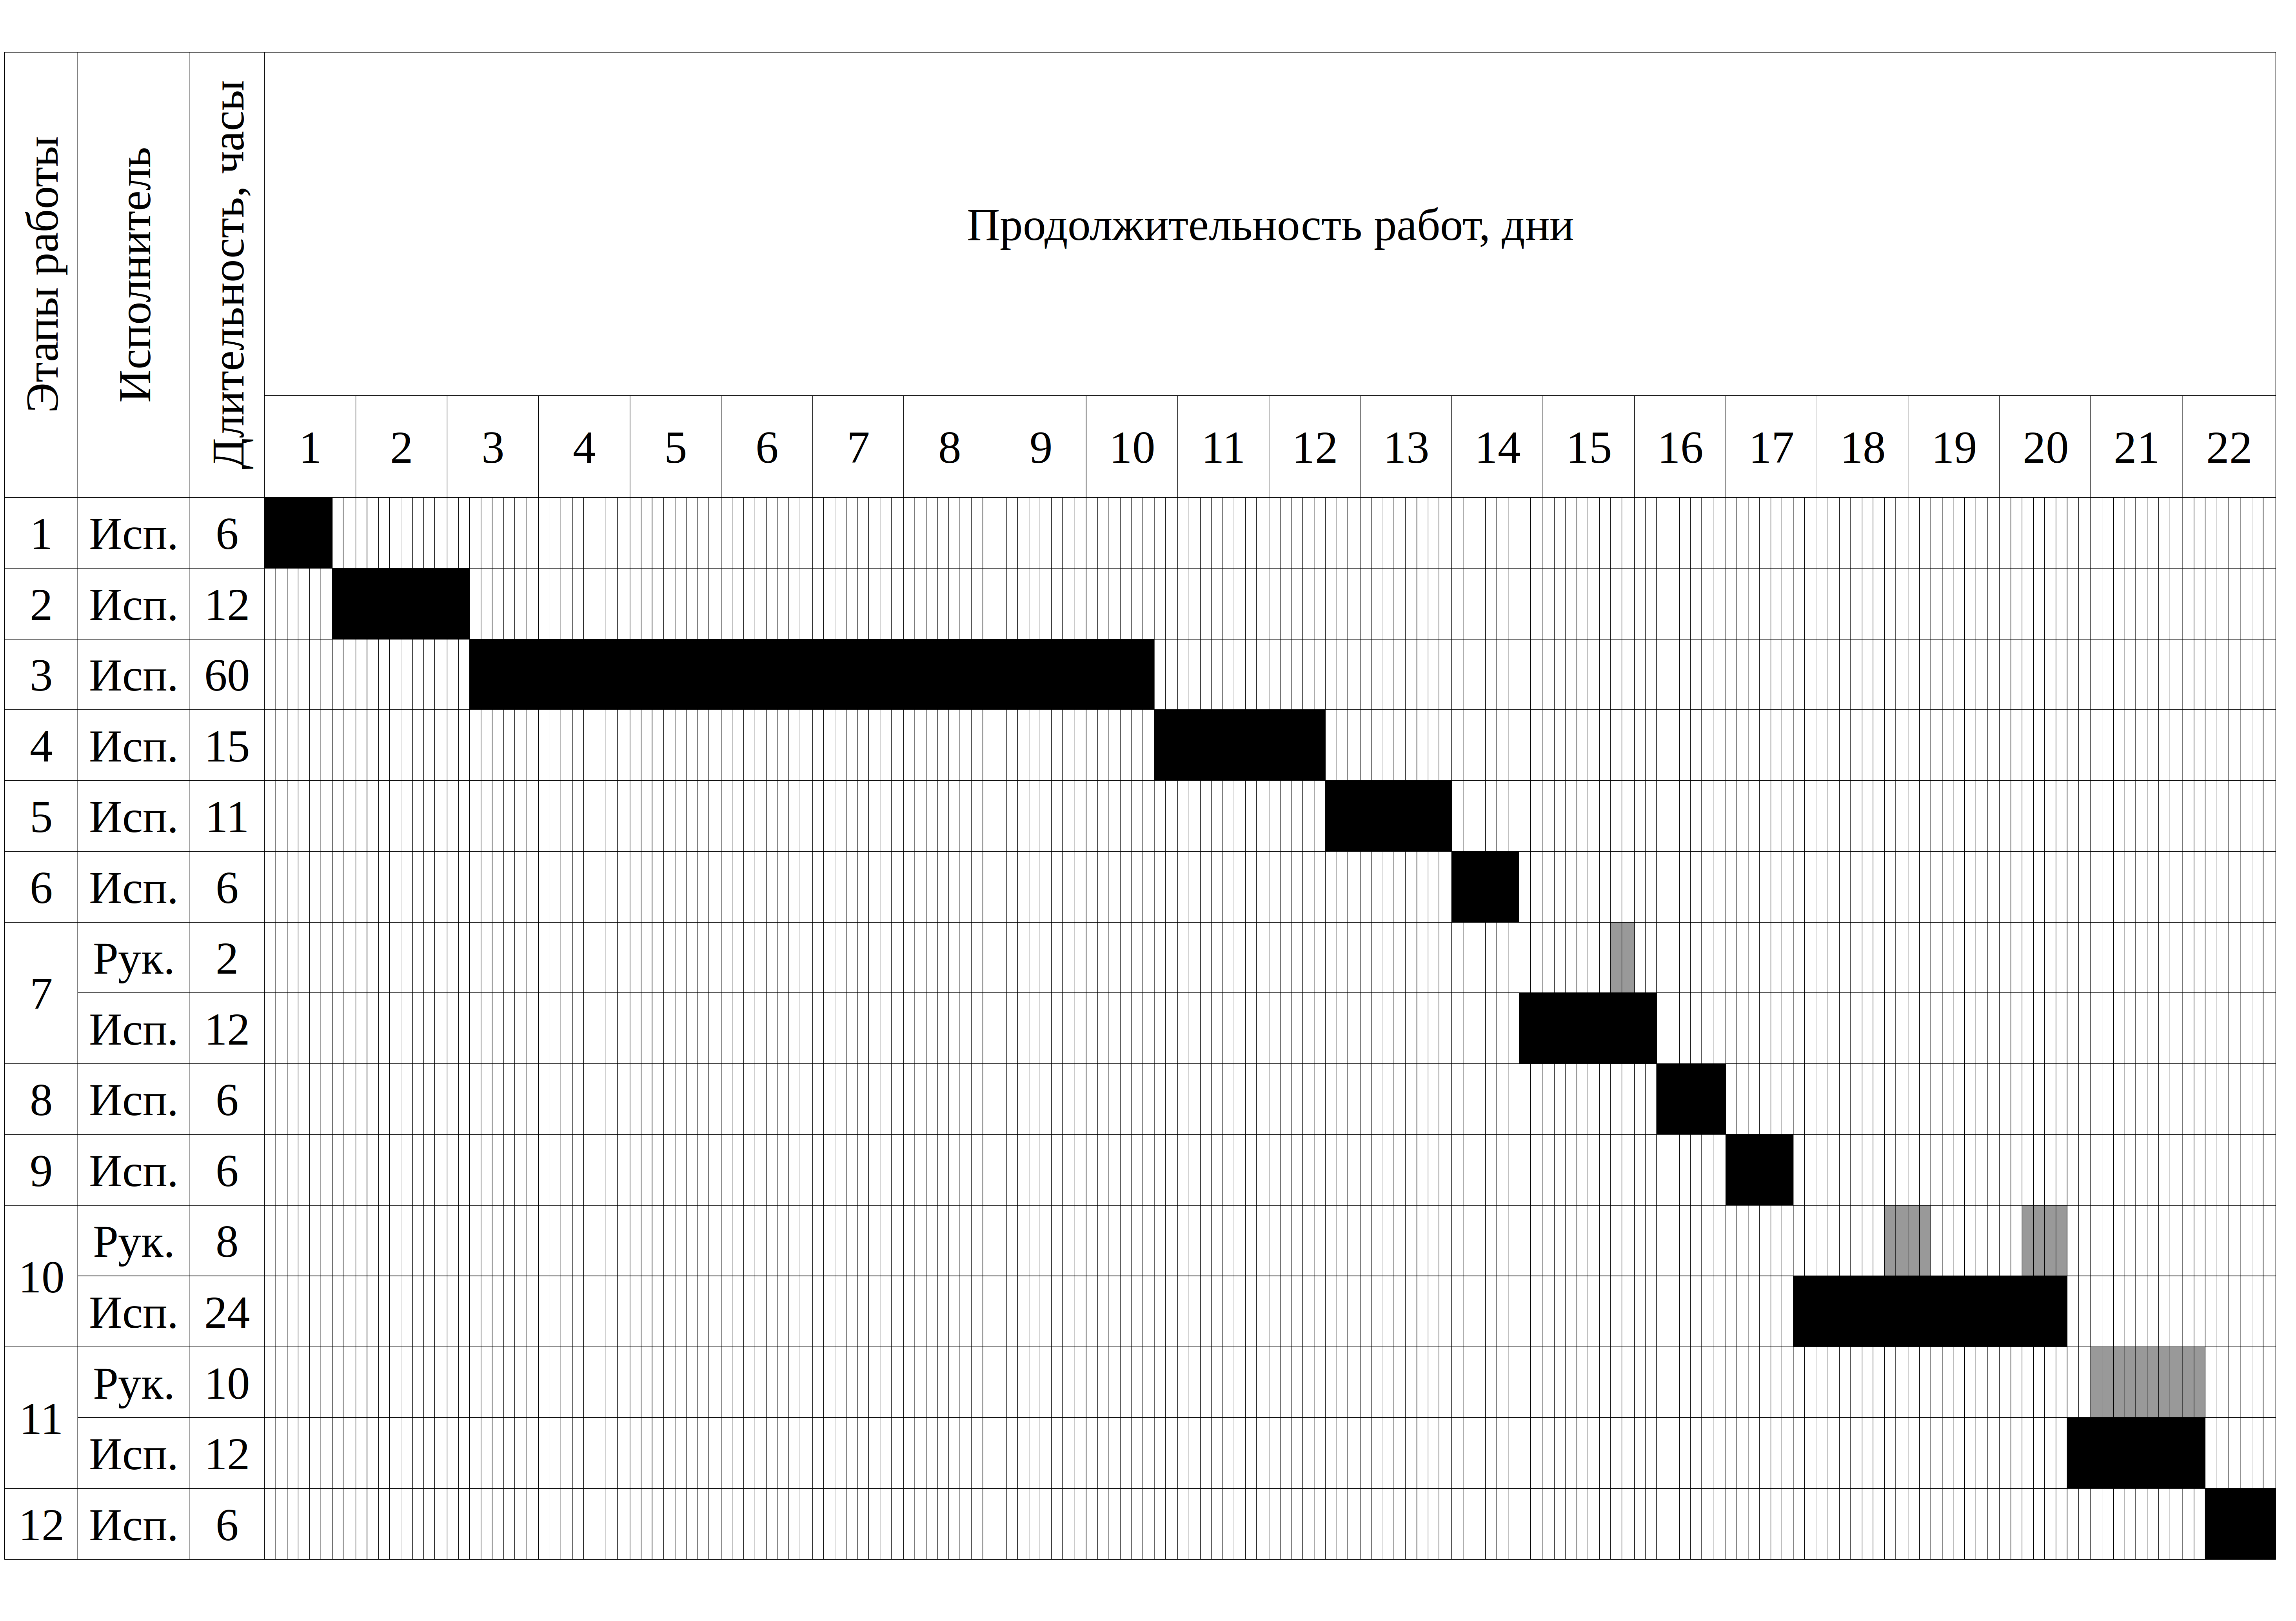
\includegraphics[width=1\linewidth]{grantt}}
\caption{ Диаграмма Ганта }
\label{grantt:grantt}
\end{figure}


На работу руководителя отводится 20 часов, исполнителя~--- 22 рабочих дня по 8 часов.

\subsection{Определение сметной стоимости работы}
\subsubsection{Затраты на оборудование и амортизацию}

Основным оборудованием при проведении работы являются компьютер и принтер, которые 
постановлением Правительства Российской Федерации от 1.01.02 г.~\textnumero~1 отнесены ко второй амортизационной группе – 
<<имущество со сроком полезного использования свыше 2 лет до 3 лет включительно>>~\cite{amort}. 

Определим норму амортизации линейным методом~\cite{frolova}. Расчет производится по формулам:

\begin{center}
 $ N_{a} = \dfrac{1}{T_{n}}\times 100\%,$
 \end{center}
 \begin{center}
 $ A = F_{n}\times N_{a}, $
\end{center}
где~~~~~ \ $N_{a}$ --- годовая норма амортизации;

$T_{n}$ --- срок полезного использования объекта основных средств;

$F_{n}$ --- первоначальная стоимость объекта основных средств;

$A$ --- сумма амортизации за год.

Годовая норма амортизации и для ноутбука, и для принтера с учетом трехлетнего срока 
использования объектов основных средств составит:
\begin{center}
$ N_{a} = \dfrac{1}{3}\times 100\% \approx 33,33\%.$\\
\end{center}

Результаты расчётов амортизационных отчислений приведены в таблице \ref{tab:job_is_done_4}.

% \clearpage
\begin{table}[!ht]
\caption{Смета затрат на амортизацию}
\centering
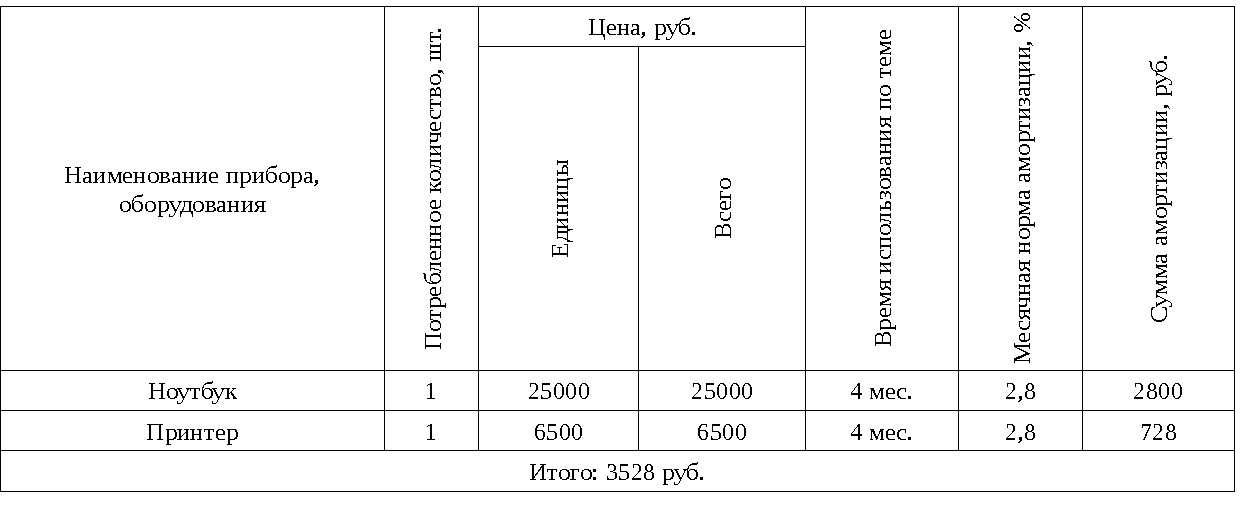
\includegraphics[page=1, width=1\linewidth]{tables/economics/schedule_4.pdf}
\label{tab:job_is_done_4}
\end{table}

Затраты на амортизацию составили 700 рублей.

\subsubsection{Расходы на оплату труда и социальные взносы}

Статья затрат учитывает выплаты по заработной плате работников, 
вычисленные на основании тарифных ставок и должностных окладов в соответствии с принятой в 
организации-разработчике системой оплаты труда. В этой статье также отражаются расчеты
премий, дополнительной заработной платы, страховых взносов.
В соответствии со статьей 426 Налогового Кодекса РФ страховые взносы составляют 30,2\%~\cite{strax} от фактической
оплаты труда.

Согласно статье 151 Трудового Кодекса РФ <<Оплата труда при совмещении профессий (должностей), 
расширении зон обслуживания, увеличении объема работы или исполнении обязанностей 
временно отсутствующего работника без освобождения от работы, определенной трудовым договором>>~\cite{tk_rf}
доплата работнику производится в случае совмещения профессий (должностей), 
расширения зон обслуживания, увеличения объема работы или исполнения 
обязанностей временно отсутствующего работника без освобождения от работы, определенной трудовым договором.

Поскольку исполнителем осуществлялась исключительно запланированная работа, дополнительная заработная
плата и премия не учитываются.

Результаты расчёта расходов на оплату труда участников работы представлены в таблице~\ref{tab:job_is_done_5}.

\begin{table}[!ht]
\caption{Расчет расходов на оплату труда участников работы}
\centering
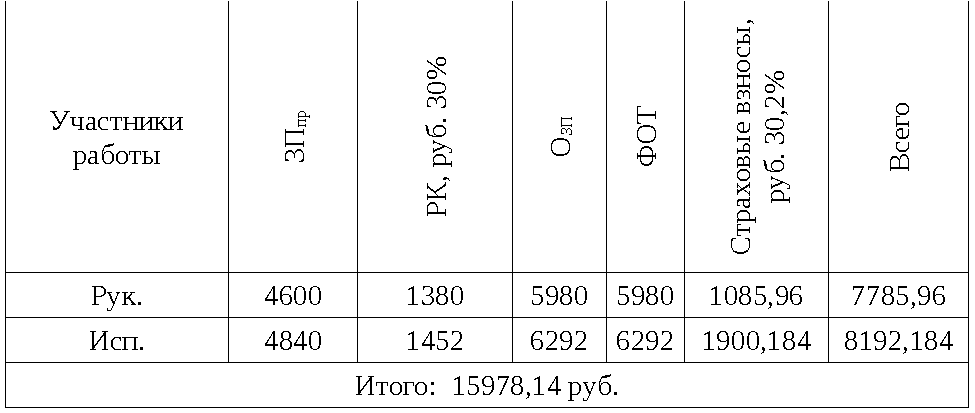
\includegraphics[page=1, width=1\linewidth]{tables/economics/schedule_5.pdf}
\label{tab:job_is_done_5}
\end{table}
Общие затраты на оплату труда участников работы составили 15978 рублей 14 копеек.


\subsubsection{Затраты на основные и вспомогательные материалы}

Статья включает расходы по приобретению и доставке основных и вспомогательных материалов, необходимых для опытно-экспериментальной проработки 
решения, для изготовления макета или опытного оборудования. Сюда включаются и стоимость необходимых материалов для изготовления образцов и 
макетов, и материалов необходимых для оформления требуемой документации.

Результаты расчёта стоимости материалов представлены в \ref{tab:eco_6}.

\begin{table}[!ht]
\caption{Расчёт затрат на основные и вспомогательные материалы}
\centering
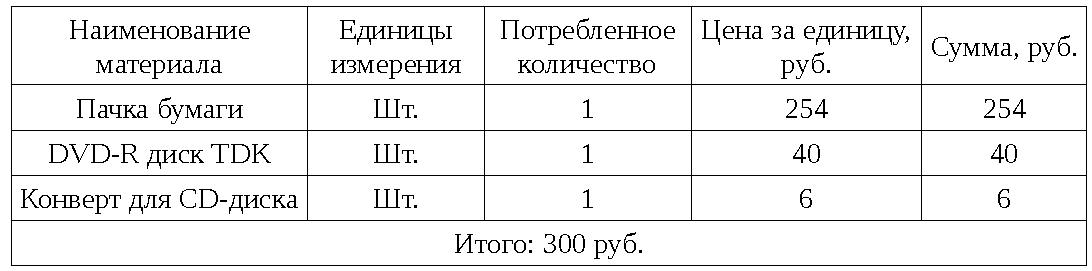
\includegraphics[page=1, width=1\linewidth]{tables/economics/econom.pdf}
\label{tab:eco_6}
\end{table}

Затраты на основные и вспомогательные нужды составили 300 рублей.

% \begin{table}[h!]
% \caption{ Расчёт затрат на основные и вспомогательные материалы }
% \label{tab:eco_6}
% \begin{center}
% \begin{tabular}{\linewidth}{|Y|Y|Y|Y|Y|}
% \hline
% Наименование материала & Единицы измерения & Потребленное количество & Цена за единицу, руб. & Сумма, руб.\\
% \hline
% Пачка бумаги & Шт. & 1 & 254 & 254\\
% \hline
% DVD-диск &Шт. & 1 & 40 & 40\\
% \hline
% Конверт для DVD-диска & Шт. & 1 & 6 & 6 \\
% \hline
% \multicolumn{5}{|c|}{Итого: 300 руб.}\\
% \hline
% \end{tabular}
% \end{center}
% \end{table}


\subsubsection{Расходы на электроэнергию}

Статья включает затраты по электроэнергии на технологические нужды. В настоящее время одноставочный
тариф на электроэнергию для населения, проживающего в городских населенных
пунктах Томской области в домах, оборудованных в установленном порядке электрическими 
плитами и (или) электроотопительными приборами,
составляет 2,17 руб./ кВт ч. Тариф введен 
Приказом от 23.12.2016 г. \textnumero~6-840 <<О тарифах на электрическую энергию для населения и 
потребителей, приравненных к категории население по Томской области на 2017 год>>~\cite{electr}, 
принятый департаментом тарифного регулирования Томской области.

Результаты расчётов приведены в \ref{tab:eco_7}.

\begin{table}[ht!]
\caption{Затраты на электроэнергию}
\centering
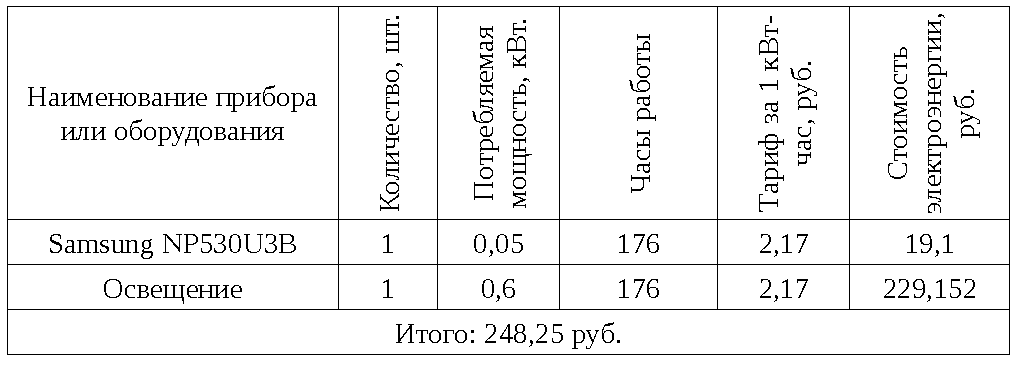
\includegraphics[page=1, width=1\linewidth]{tables/economics/econom_2.pdf}
\label{tab:eco_7}
\end{table}

Затраты на электроэнергию составили 248 рублей 25 копеек.


\subsubsection{Накладные расходы}

Результаты расчёта накладных расходов приведены в таблице~\ref{tab:eco_8}.

\begin{table}[ht!]
\caption{Накладные расходы}
\centering
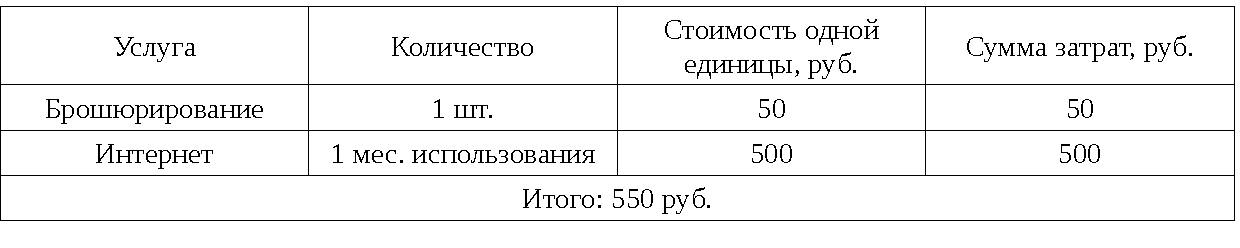
\includegraphics[page=1, width=1\linewidth]{tables/economics/econom_3.pdf}
\label{tab:eco_8}
\end{table}

Накладные расходы составляют 550 рублей.


\subsubsection{Сводная смета затрат}

На основании всех произведённых расчётов составим сводную смету затрат на выполнение работы в виде таблицы \ref{tab:eco_9}.

\begin{table}[ht!]
\caption{Сводная смета затрат}
\centering
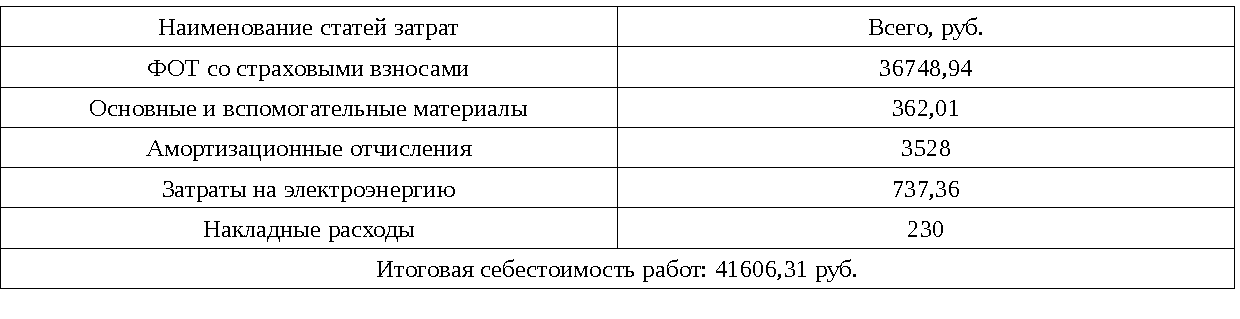
\includegraphics[page=1, width=1\linewidth]{tables/economics/econom_4.pdf}
\label{tab:eco_9}
\end{table}

Итого общая сумма затрат на выполнение дипломной работы составила 17776,39 рублей.
Около 90\% всех расходов приходится на оплату труда руководителя и исполнителя, остальные 10\% --- 
на прочие расходы, включающие в себя амортизацию, расходы на электроэнергию, основные и вспомогательные
материалы, а также накладные расходы.


%%%%%%%%%%%%%%%%%
%  \newpage
%  \renewcommand{\refname}{Список использованных источников}
% %  \addcontentsline{toc}{section}{Список использованных источников}
%  \bibliography{lit}
% \end{document}